\documentclass[11pt,a4paper,titlepage]{report} 
\usepackage[utf8]{inputenc} 
\usepackage[french]{babel} 
\usepackage[T1]{fontenc} 
\usepackage{amsmath} 
\usepackage{amsfonts} 
\usepackage{amssymb} 
\usepackage{graphicx} 
\usepackage[final]{pdfpages} 
\usepackage[toc,page]{appendix} 
\usepackage[top=2.5cm,bottom=2.5cm,right=2.5cm,left=2.5cm]{geometry} 

\newcommand{\HRule}{\rule{\linewidth}{0.5mm}}

\begin{document}
\renewcommand{\thefootnote}{\fnsymbol{footnote}}
\begin{titlepage}
\begin{center}

% Upper part of the page. The '~' is needed because \\
% only works if a paragraph has started.
%
\includegraphics[width=0.15\textwidth]{./logo}~\\[1cm]

\includegraphics[width=0.15\textwidth]{logo.png}~
\\[1cm]
\textsc{\LARGE iut informatique de belfort-montbéliard}\\[1cm]

\textsc{\Large Projet de base de données}\\[0.5cm]

% Title
\HRule \\[0.4cm]
{ \huge \bfseries Velacampus website \\[0.4cm] }

\HRule \\[1.5cm]

% Author and supervisor
\begin{minipage}{0.4\textwidth}
\begin{flushleft} \large
\emph{Auteur:}\\
Morgane \textsc{cabrol}\\
Pierre \textsc{limballe}\\
Geoffrey \textsc{glangine}\\
Auguste \textsc{meyer}
\end{flushleft}
\end{minipage}
\begin{minipage}{0.4\textwidth}
\begin{flushright} \large
\emph{Superviseur:} \\
Alexandru  \textsc{dobrila}
\end{flushright}
\end{minipage}

\vfill

% Bottom of the page
{\large \today}

\end{center}
\end{titlepage}

\tableofcontents
\chapter*{Introduction}
Vélocampus est une association louant des vélos aux étudiants à très petit tarifs. De plus, elle s’occupe de la réparation et de l'entretien de vélos loués ou non.

Pour ce projet, nous avons voulu réaliser un site permettant à Vélocampus de gérer son administration plus facilement. Pour cela nous vous présenteront d'abord le cahier des charges que nous avons conçus avec les membres de l'association, puis nous expliquerons la base de données que nous avons décidés de mettre en place, ainsi que les fonctionnalités que nous avons implémenté sur le site. Enfin, nous aborderons les problèmes que nous avons rencontrés puis, les améliorations qui pourraient être apporté au site par la suite.


\chapter{Le cahier des charges}
Après une réunion avec les membres de l'association, nous sommes arrivés à la conclusion que le site contiendrait une petite partie client, rendant ainsi l'association présente sur le web et une grosse partie administration, permettant toutes la gestions de l'association. 
Nous avons finalement construit ce cahier des charges :\\


\section{La partie administration :} 
Elle sera accessible à tous les membres de l'association \\
\begin{itemize}
\item Une mailing liste des adhérents \\
\textit{(Permettant à l'administrateur d'importer la liste sur une boite mail afin de pouvoir envoyer des messages groupés)}
\item Un Suivi des vélos \\
\textit{(Afin de savoir quel vélo est en location, quel vélo a subit quel réparation...)}
\item Une gestion des demandes d'adhésions faites en lignes 
\item Une messagerie internet \\
\textit{(Permettant aux différents administrateurs de communiquer entre eux)}
\item Une gestion des vélos \\
\textit{(Pour ajouter des vélos, supprimmer des vélos ou encore modifoer des vélos)}
\item Une gestion de réparation \\
\textit{(Permettant d'ajouter des réparations à certain vélo et de connaitre le prix de ces réparations)}
\item Une gestion du site publique \\
\textit{(Ajouter des photos, modifier les partenaires, modifier le messages d'acceuil ...)}
\item L'importation d'un calendrier Gmail \\
\textit{(Permettant d'importer un calendrier d'évenement sur la partie client du site et d'afficher le calendrier interne de l'association sur la partie administration du site)}
\end{itemize}

  
  
\section{ La partie client :}

\begin{itemize}
\item Une formulaire d'adhésion \\
\textit{(Permettant aux visiteurs de s'inscrire en ligne)}
\item Un formulaire de demande de réparation \footnote{Cette partie n'est accessible que par les adhérents connectés}  \\
\textit{(Permettant aux adhérents de demander la réparations de leurs vélos )}
\item Calendrier en ligne avec les événements de l'association 
\item Une page d'informations  \\
\textit{(Contenant la présentations de l'association, ses membres et ses partenaires)} 
\item Une page de photos et videos  

\end{itemize}
\chapter{Base de données}
\section{le modèle conceptuel de donnée}
\begin{center}
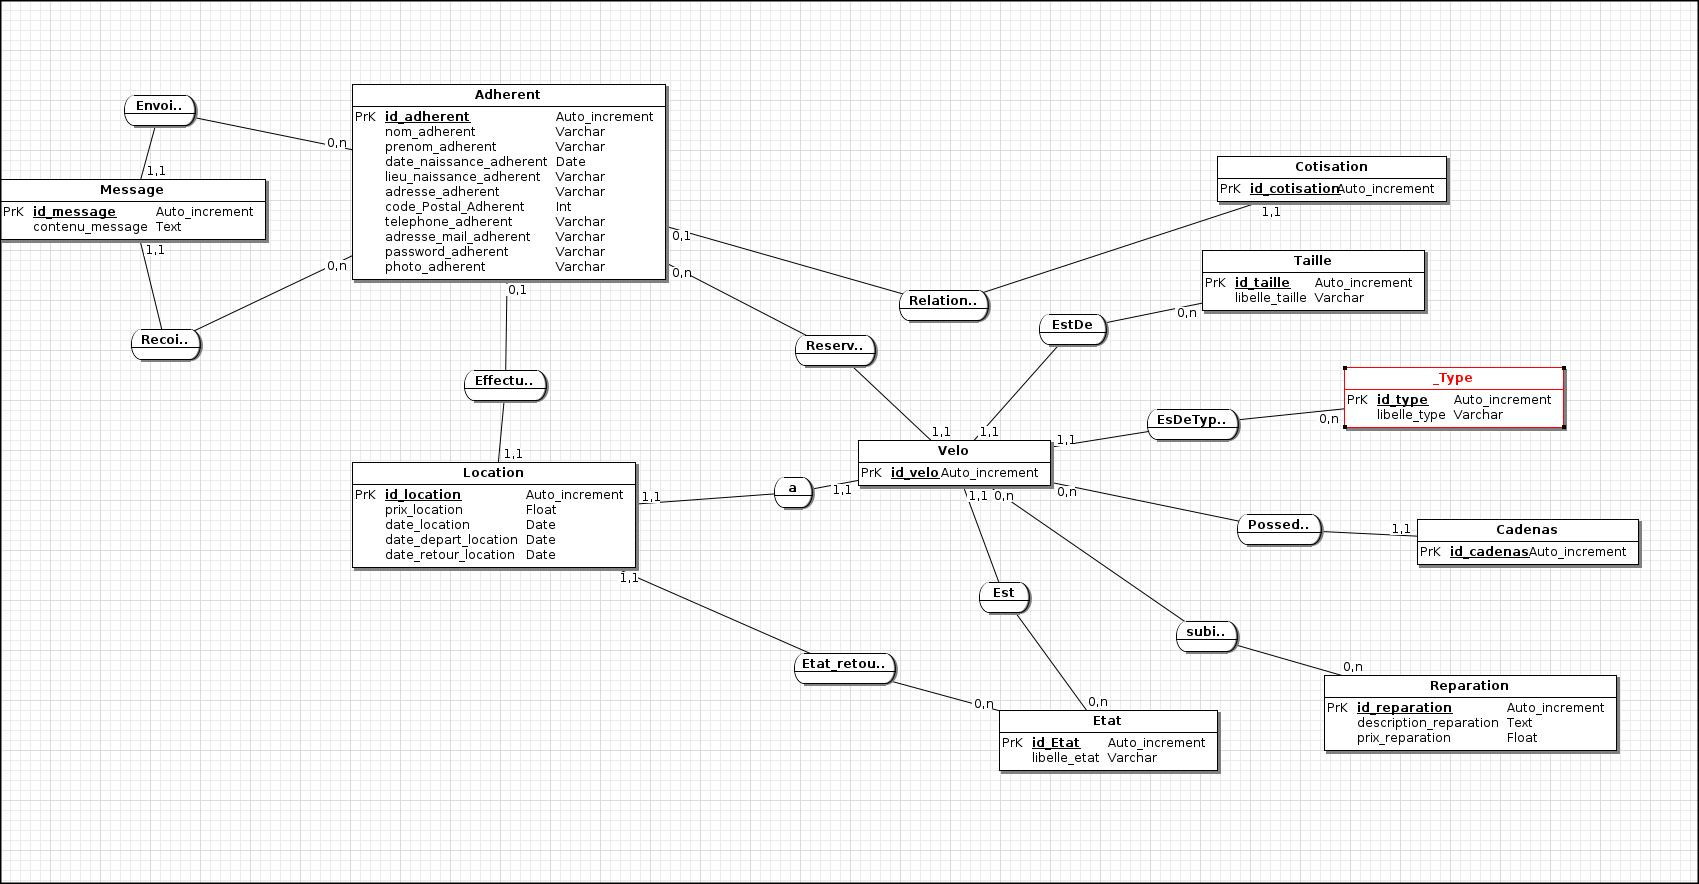
\includegraphics[width=1\textwidth]{MCD.jpg}~
\end{center}

\section{La réalisation du MCD}

\chapter{Le fonctionnement du site Internet}


\chapter{Les problèmes rencontrés}
\begin{itemize}
\item Adblock bla bla bla
\item Chemin absolut bla bla bla
\item Repartition du travail bla bla bla
\item ??
\end{itemize}
\chapter{Les améliorations possibles}
\begin{itemize}
\item Réparation d'un vélo non loué bla bla bla
\item Demande de location en ligne bla bla
\item Gestion des compte rendu de reunions bla bla
\item Ajout d'un forum bla bla
\item Ajout d'une fontionnalité de paiement en ligne bla bla
\end{itemize}
\chapter*{Conclusion}
\end{document}



